\section{Vincoli}
  \subsection*{ Vincoli tecnologici}

  Il piano di lavoro tramite gli obiettivi, intrinsecamente, ha definito i vincoli tecnologici del progetto.\\
  Il primo vincolo è stato quello di utilizzare un \textit{database} a grafo per il salvataggio dei dati raccolti dal \textit{plugin},
  questo perchè permette di rappresentare le dipendenze in maniera naturale, e di eseguire \textit{query} molto complesse in tempi molto brevi.\\
  Con i membri del team abbiamo deciso di utilizzare Neo4j come \textit{database} a grafo, perchè è il più utilizzato, ha una comunità molto attiva
ed è molto ben documentato.

Il secondo vincolo tecnologico è stato quello di utilizzare Gradle per il \textit{plugin} che raccoglie le informazioni sulle dipendenze,
questo perchè quasi tutti i progetti di {\azienda} lo utilizzano come sistema di \textit{build}.\\

\subsubsection*{Gradle}
  Gradle è uno strumento di automazione della \textit{build} \textit{open source} che si è guadagnato una notevole popolarità nel mondo 
dello sviluppo \textit{software}, grazie alla sua flessibilità e potenza. Utilizzato principalmente per progetti Java, 
è anche ampiamente adottato per applicazioni scritte in altri linguaggi di programmazione come Kotlin, C++, e \textit{Python}. 
La sua caratteristica principale è la capacità di supportare configurazioni di \textit{build} altamente personalizzabili, 
rendendolo adatto sia per piccoli progetti sia per grandi imprese con esigenze complesse.

Gradle si distingue per l'uso di un \gls{DSLg} basato sui linguaggi di programmazione \textit{Groovy} o Kotlin,
 che fornisce un modo intuitivo e dichiarativo di definire le \textit{build}. Questo approccio, combinato con la sua potente capacità di 
 gestione delle dipendenze e il suo modello di esecuzione incrementale, consente agli sviluppatori di costruire \textit{software} in modo più 
 efficiente e affidabile. Inoltre, Gradle è noto per la sua velocità, superando spesso altri strumenti di \textit{build} come Maven 
 e \textit{Ant}, specialmente in progetti di grandi dimensioni, la figura \ref*{fig:gredle-vs-maven} mostra alcune differenze in termini di velocità 
 tra Gradle e Maven.

 \begin{figure}[!h] 
  \centering 
  \includegraphics[width=1\columnwidth]{Gradle-vs-maven.jpeg} 
  \caption[Confronto tra Gradle e Maven]{Confronto tra Gradle e Maven. Fonte: \url{https://Gradle.org/maven-vs-Gradle}}
  \label{fig:gredle-vs-maven}
\end{figure}

Un altro aspetto fondamentale di Gradle è la sua estensibilità. Gli sviluppatori possono estendere le funzionalità di Gradle 
scrivendo script personalizzati o integrando \textit{plugin} esistenti. Questa flessibilità lo rende uno strumento ideale per adattarsi a 
flussi di lavoro specifici e requisiti di \textit{build} unici. Gradle è anche il sistema di \textit{build} ufficiale per Android, ulteriormente 
consolidando la sua posizione come uno strumento chiave nello sviluppo di applicazioni moderne.

\subsubsection*{Angular}
Un altro vincolo tecnologico è stato quello di utilizzare Angular per lo sviluppo del \textit{frontend}, 
questo perchè, come scritto precedentemente, è il \textit{framework} più utilizzato in azienda per lo sviluppo delle \textit{web-app}.\\

Angular è un \textit{framework} \textit{front-end} \textit{open source} sviluppato e mantenuto da Google. 
È ampiamente riconosciuto per la sua capacità di creare applicazioni \textit{web} dinamiche e reattive. \\
Angular utilizza TypeScript, una \textit{super-set} di JavaScript, che fornisce funzionalità di tipizzazione statica e 
orientamento agli oggetti, migliorando la manutenibilità e la qualità del codice.

Una delle caratteristiche distintive di Angular è il suo approccio basato su componenti, che aiuta gli sviluppatori a 
costruire applicazioni \textit{web} complesse in modo più modulare e mantenibile. Ogni componente in Angular è una combinazione di \textit{HTML}, 
CSS, e TypeScript, che gestisce una parte specifica dell'interfaccia utente. Questo approccio promuove la riusabilità 
del codice e una migliore separazione delle preoccupazioni.

Angular è anche noto per il suo potente sistema di \textit{dependency injection}, che semplifica lo sviluppo e il \textit{testing} fornendo un 
modo per iniettare dipendenze in classi in modo pulito e flessibile. Inoltre, offre un'ampia gamma di funzionalità integrate come il 
\textit{routing}, la gestione delle \textit{form}, e l'accesso HTTP, che accelerano lo sviluppo di applicazioni \textit{web}.

\begin{figure}[h] 
  \centering 
  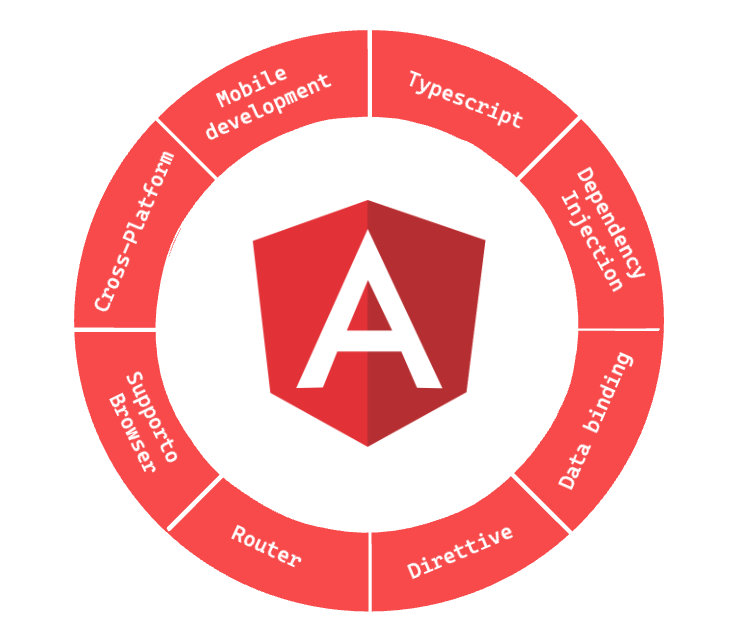
\includegraphics[width=0.5\columnwidth]{feature-angular.png} 
  \caption{Caratteristiche di Angular.}
  \label{fig:feature-angular}
\end{figure}

Con il suo ecosistema ricco (figura \ref*{fig:feature-angular}) e una forte comunità di sviluppatori, Angular è diventato uno dei \textit{framework} \textit{front-end} più popolari e 
affidabili per lo sviluppo di applicazioni \textit{web} moderne, sia per progetti di piccole dimensioni sia per applicazioni aziendali di grande scala.

\subsubsection*{I \textit{database} a grafo e Neo4j}

I \textit{database} a grafo sono una categoria di \textit{database} NoSQL progettati per gestire e rappresentare dati complessi e le loro relazioni 
in modo più efficiente rispetto ai tradizionali \textit{database} relazionali, la figura \ref*{fig:graphdb-vs-sql} mostra alcune differenze tra i \textit{database} relazionali e quelli a grafo.\\
Questi \textit{database} utilizzano strutture di grafo per la memorizzazione 
semantica, con nodi, bordi e proprietà per rappresentare e memorizzare dati. La flessibilità dei \textit{database} a grafo li rende particolarmente 
adatti per applicazioni che richiedono l'analisi di relazioni complesse e interconnesse, come i \textit{social network}, i sistemi di raccomandazione, 
e la gestione delle reti.

Neo4j è uno dei più popolari \textit{database} a grafo, noto per la sua alta \textit{performance} e flessibilità. È un \textit{database} 
\textit{open source}, ma offre anche una versione \textit{enterprise} con funzionalità aggiuntive. Neo4j utilizza il linguaggio di 
\textit{query} Cypher, che è specificamente progettato per lavorare con grafi. Cypher consente agli sviluppatori di esprimere 
facilmente \textit{query} complesse sulle relazioni tra i dati, rendendo Neo4j particolarmente potente per analisi di dati relazionali complessi.

\begin{figure}[h] 
  \centering 
  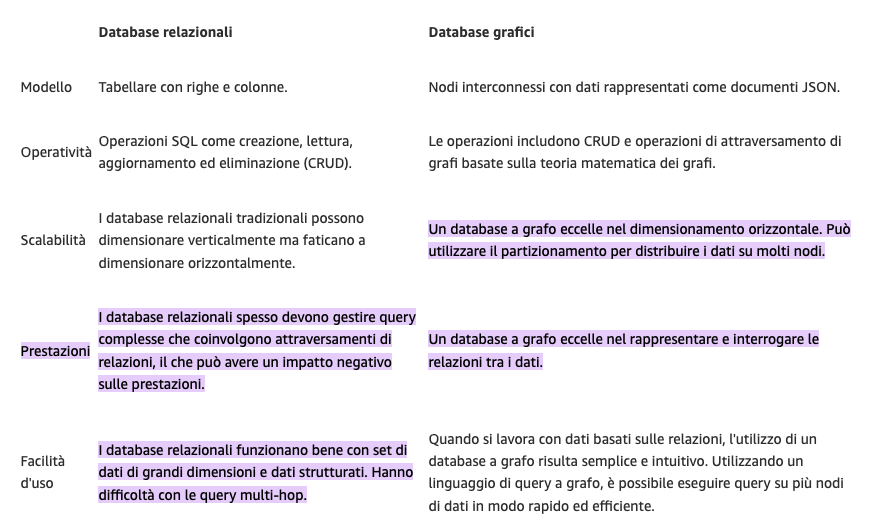
\includegraphics[width=1\columnwidth]{graphdb-vs-sql.png} 
  \caption[Differenze tra \textit{database} a grafo e \textit{database} relazionali.]{Differenze tra \textit{database} a grafo e \textit{database} relazionali. \\Fonte: \url{https://aws.amazon.com/it/compare/the-difference-between-graph-and-relational-database}.}
  \label{fig:graphdb-vs-sql}
\end{figure}

\subsection*{ Vincoli di dominio}
Il prodotto finale dovrà essere utilizzato, non solo dagli sviluppatori, ma anche dai \textit{project manager}, i \textit{team leader},
 i \textit{product owner} ed i consulenti; 
 Per questo è stato richiesto, come obiettivo desiderabile, di implementare l'autenticazione tramite \textit{LDAP} aziendale, 
per permettere l'accesso a tutti i dipendenti di {\azienda}.\\
L'\textit{LDAP} è un protocollo di rete che permette la gestione centralizzata delle autenticazioni e delle autorizzazioni.
Questo è fondamentale per garantire la sicurezza dei dati, e per permettere l'accesso solo a chi ne ha i permessi, senza dover
implementare un sistema di autenticazione ad hoc.\\
